In this phase we defined the review protocol. This protocol contains: (\textit{i}) the research questions, (\textit{ii}) the search strategy, (\textit{iii}) the inclusion and exclusion criteria and (\textit{iv}) the data extraction and synthesis method.

%Research questions must embody the review study purpose. Moreover, these questions reflect the general scope of the review study. The scope is comprised of population (i.e., population group observed by the intervention), intervention (i.e., what is going to be observed in the context of the planned review study), and outcomes of relevance (i.e., the results of the intervention). Furthermore, during the conduction of this step, it was also necessary to establish the scope of the review study. According to the systematic review process~\cite{Kitchenham}, the scope has to be established using the PICO criteria. Thus, herein our \textbf{Population} is published scientific literature reporting on the use of Architecture-Driven Modernization and its metamodels. The \textbf{Intervention} is published scientific literature interested with Architecture-Driven Modernization and its metamodels. The \textbf{Comparison} is not applied herein. Finally, the \textbf{Outcomes of relevance} is an overview of the studies that have been conducted in the field of Architecture-Driven Modernization and its metamodels, emphasizing primary studies that report on the process used in the research area, from observing such an aggregated data set, we also intend to provide insight into the frequencies of publication over time to inspect trends.   

%\begin{itemize}

%\item \textbf{Population:} published scientific literature reporting on some existing mining techniques for crosscutting concern.

%\item \textbf{Intervention:} published scientific literature concerned with mining techniques for crosscutting concern. Furthermore, we also aim at determining which techniques are the most used within academic settings.

%\item \textbf{Comparison:} No applied herein.

%\item \textbf{Outcomes of relevance:} an overview of the studies that have been conducted in the field of crosscutting concern mining, emphasizing primary studies that report on the techniques used in the research area. From observing such an aggregated data set we also intend to provide insight into the frequencies of publication over time to inspect trends.

%\end{itemize} 

%Como ADM esta sendo aplicada na literatura para auxiliar a modernizacao de sistemas legados

The objective of this review is to find out \textbf{how ADM has been applied in the literature to assist engineers during the process of modernization of legacy systems}. In order to achieve such objective we formulated five research questions. \textbf{RQ$_1$:} What are the focus area most discussed and least discussed in the literature regarding the ADM? Moreover, what types of contributions have been presented so far?; \textbf{RQ$_2$:} Given the ADM's standards metamodels, which one has been more used in the literature? In addition, given the identified metamodel, what are the packages most and least used?; \textbf{RQ$_3$:} Which research types have been employed into the field herein?; \textbf{RQ$_4$:} Which are the existing tool support for ADM? Moreover, how the tools perform the identification of what needs to be modernized?

%\begin{description}

%\item[\textbf{RQ$_1$:}] What are the focus area most discussed and least discussed in the literature regarding the ADM? Moreover, what types of contributions have been presented so far?

%\item[\textbf{RQ$_2$:}] Given the ADM's standards metamodels, which one has been more used in the literature? In addition, given the identified metamodel, what are the packages most and least used?

%\item[\textbf{RQ$_3$:}] Which research types have been employed into the field herein?

%\item[\textbf{RQ$_4$:}] Which avenues are often used to publish research related to ADM?

%\item[\textbf{RQ$_5$:}] Which are the existing tool support for ADM? Moreover, how the tools perform the identification of what needs to be modernized?



%\item[\textbf{RQ$_4$:}] Given a set of concerns, which are the most indicated techniques for performing the mining?

%\item[\textbf{RQ$_5$:}] How can someone combine the techniques for improving the precision and recall metrics?

%\item[\textbf{RQ$_3$:}]  Considering the techniques that we found, which ones have automated support?

%\end{description}

To address \textbf{RQ$_1$}, we read all primary studies in order to identify the focus area of each study. Next, we arrange all studies according to the focus area. Whether any kind of disagreement related to the focus area that the article meets, it was marked and was discussed with everyone involved in the review in order to clarify which topic it belongs. With respect to \textbf{RQ$_2$}, we also read all primary studies and identified which metamodel was used in the study. With respect to \textbf{RQ$_3$}, we used and adapted the scheme proposed by Wieringa et al~\cite{Wieringa:2005:REP:1107677.1107683} in order to classify each primary study into a research type, see Section~\ref{research_type}. Finally, to address \textbf{RQ$_4$} we read all primary studies in order to identifiy the tools used to modernize the legacy systems. %Next, we arrange the identified tools according to the focus area. 


Afterwards, we defined the search string and chose the electronic databases. The search string was created based upon a set of keywords. Figure~\ref{search_string} shows the search string elaborated. The search encompassed electronic databases which are deemed as the most relevant scientific sources~\cite{Kitchenham} and therefore likely to contain important primary studies. We used the search string on the following electronic databases: \textit{ACM}, \textit{IEEE XPLORE}, \textit{Scopus}, \textit{Web of Science} and \textit{Engeneering Village}. Note that since the features provided by various databases, as well as the exact syntax of search strings to be applied vary from one database to other, the string given in Figure~\ref{search_string} was actually used to construct a semantically equivalent string specific to each database.

%Furthermore, no limits were placed on date of publication with a view to not restrict the review study scope. %Aimed at keeping track of the selected papers, we used JabRef\footnote{http://jabref.sourceforge.net/}, an open source system for bibliography reference management. 

\begin{figure}[!h]
\centering
  % Requires \usepackage{graphicx}
  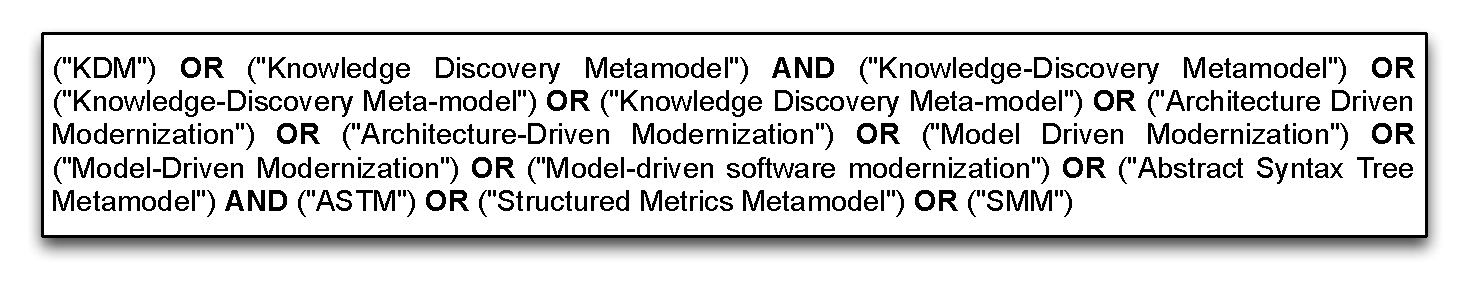
\includegraphics[scale=0.35]{figuras/SearchStringADM}
\caption{Search String.}
\label{search_string}
\end{figure} 

Then, in order to determine which primary studies are relevant to answer our research questions, we applied a set of inclusion and exclusion criteria. Inclusion criteria applied were: (\textit{i}) \textbf{The primary study presents at least one solution of modernization by means of ADM} - (\textit{ii}) \textbf{Studies that explicitly present an ADM approach} - (\textit{iii}) \textbf{The primary study presents at least one type of evaluation technique for ADM}. 
%\begin{enumerate}[(a)]%for small alpha-characters within brackets.
%\item \textbf{The primary study presents at least one solution of modernization by means of ADM:} the paper provides evidences that the ADM assists the software engineer during the modernization/refactoring of legacy system.

%\item \textbf{Studies that explicitly present an ADM approach:} the paper provides an approach to assist the software engineer to modernize the legacy system.

%\item \textbf{The primary study presents at least one type of evaluation technique for ADM:} without the results of the evaluation we would not be able to make comparisons desired. In other words, the paper must clearly present which assessment techniques have been employed to evaluate the ADM process, i.e., case study, experiment, survey, etc.

%\end{enumerate}
Not all of these criteria must be present for every primary study. However, at least the former, i.e., (a), must be present. If all criteria were mandatory, the number of selected techniques would decrease significantly.

Exclusion criteria applied were: (\textit{i}) \textbf{Papers which mentioned ADM and its metamodels only in the abstract} - (\textit{ii}) \textbf{Introductory papers for books and workshops} and (\textit{iii}) \textbf{The primary study is a short paper}. We elaborated data extraction forms to accurately record the information obtained by the researchers from the primary studies. The form for data extraction provides some standard information, such as (\textit{i}) a brief of the primary study, highlighting where ADM and its metamodels were used, (\textit{ii}) date of data extraction, (\textit{iii}) title, authors, journal, publication details and (\textit{iv}) a list of each conclusion and statement encountered for each question. 

During the extraction process, the data of each primary study were independently gathered by three reviewers. The review was performed in August, 2013 by two M.Sc. and a Ph.D. student. All the results of the search process are documented in the web material(tinyurl.com/99spmaz). So, it is clear to others how thorough the search was, and how they can find the same documents.
